\documentclass[12pt]{article}
\usepackage[a4paper]{geometry}
\usepackage{fullpage}
\usepackage[T1]{fontenc}
\usepackage[utf8]{inputenc}
\usepackage{graphicx}
\usepackage{mathpazo}
\pagenumbering{gobble}
\usepackage{siunitx}
\sisetup{output-decimal-marker = {,}}
\usepackage{amsmath}
\usepackage{esdiff}
\usepackage[spanish]{babel}
\usepackage{cancel}
\newcommand{\laplace}[1]{\mathbf{#1}(\mathbf{s})}
\newcommand{\slp}{\mathbf{s}}

\begin{document}

\title{\textsc{Teoría de Circuitos III}\\Prueba BT5 (Turno 2)}

\date{21 de enero de  2019\\\small{Los resultados se publicarán el 22 de enero.\\La revisión del examen se realizará los días \textbf{23 y 24} de enero de 2019 de \textbf{11:30 a 13:30}.}}

\maketitle

El circuito de la figura representa una fuente de corriente alterna sinusoidal alimentando dos cuadripolo $Q_1$ idénticos conectados en cascada, y una impedancia de carga. 
\begin{enumerate}

\item Determina los parámetros de transmisión del cuadripolo $Q_1$.

\item Determina los parámetros de transmisión del cuadripolo equivalente, $Q_T$, conformado por la asociación de los dos cuadripolos $Q_1$. Calcula la impedancia de entrada del cuadripolo $Q_T$ y obtén la impedancia que debe tener el generador para se produzca máxima transferencia de potencia.

\item ¿Cuál es la impedancia de \textbf{salida} del cuadripolo $Q_T$ si la impedancia de la fuente que lo alimenta es la obtenida en el apartado anterior?

\item Determina la impedancia que habría que conectar a la salida de $Q_T$ en lugar de $\overline{Z}_L$ para que desde la entrada de $Q_T$ se observe esa misma impedancia. En estas condiciones, ¿que relación de atenuación hay entre los valores eficaces de las tensiones de entrada y salida del cuadripolo $Q_T$?.

\end{enumerate}


\begin{minipage}{0.2\textwidth}
  Datos:
  \begin{itemize}
  \item $R$ = \SI{1}{\ohm}
  \item $X_C$ = \SI{2}{\ohm}
  \item $\overline{Z}_L$ = -j\SI{2}{\ohm}
  \end{itemize}
\end{minipage}
\begin{minipage}{0.8\textwidth}
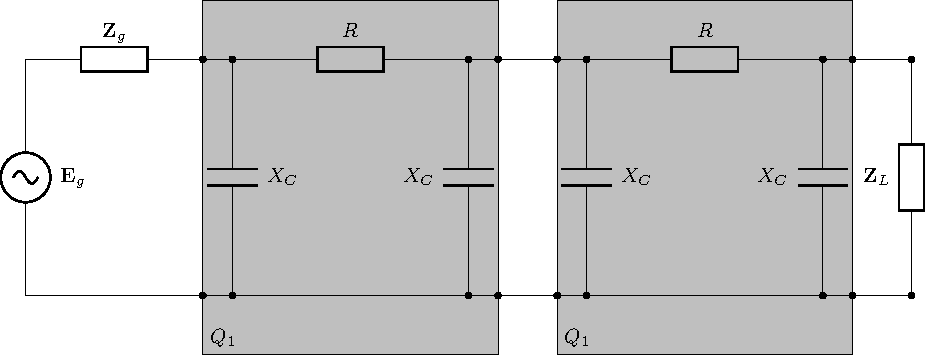
\includegraphics[scale=0.85]{figs/E5_circuito2.pdf}
\end{minipage}

\clearpage 
\subsection*{Solución}

\begin{enumerate}
\item Parámetros impedancia

  Para obtener los parámetros impedancia se pueden aplicar
  directamente las ecuaciones de esta familia. Otra opción es obtener
  los parámetros admitancia, dado que se trata de un circuito $\pi$, y
  transformar a parámetros de transmisión. En cualquier caso, el
  resultado es:

\[
  [\overline{T}] = \left[
    \begin{array}{cc}
      1 + 0.5j & 1\\
      -0.25 + j & 1 + 0.5j\\
    \end{array}
  \right]
\]

Comprobamos que la matriz cumple las propiedades de un circuito
recíproco y simétrico.

 
\item Asociación en cascada

  \[
    [\overline{T}_{QT}] = [\overline{T}_1] \cdot [\overline{T}_1] = \left[
      \begin{array}{cc}
        0.5 + 2j & 2 + j\\
        -1.5 + 1.75j & 0.5 + 2j\\
      \end{array}
    \right]
  \]
  

  
  La impedancia de entrada en función de los parámetros transmisión se
  expresa:

\[
  \overline{Z}_i = \frac{\overline{A} \overline{Z}_L +
    \overline{B}}{\overline{C}\overline{Z}_L + \overline{D}}
\]

Sustituyendo valores obtenemos:

  \[
    \overline{Z}_{i} = \SI[parse-numbers=false]{0.585 - 0.732j}{\ohm}
  \]

  Por tanto, para que se produzca máxima transferencia de potencia, la
  impedancia del generador debe ser:

  \[
    \overline{Z}_{g} = \overline{Z}_{i}^* = \SI[parse-numbers=false]{0.585 + 0.732j}{\ohm}
  \]
\item Impedancia de salida

  La impedancia de salida de un cuadripolo a partir de los parámetros de transmisión se calcula con la siguiente expresión:

\[
  \overline{Z}_{out} = \frac{\overline{D} \cdot \overline{Z}_{g} +
    \overline{B}}{\overline{C} \cdot \overline{Z}_{g} + \overline{A}}
\]

  \[
    \overline{Z}_{out} = \SI[parse-numbers=false]{0.543 - 0.898j}{\ohm}
  \]
\item Se trata de conectar la impedancia característica del cuadripolo:

  \[
    \overline{Z}_o = \sqrt{\frac{B}{C}} = \SI[parse-numbers=false]{0.606-0.776j}{\ohm}
  \]

  Al conectar esta impedancia, la relación entre las tensiones de entrada y salida está definida por la constante de propagación:

  \[
    \exp{\overline{\gamma}} = \overline{A} + \sqrt{\overline{A}^2 - 1} = 0.949 + 4.225j
  \]

  La relación de atenuación de los valores eficaces de tensión se determina con la parte real de $\overline{\gamma} = \alpha + j\beta$:

  \[
    \exp{\alpha} = \frac{U_1}{U_2} = 4.33
  \]
  
\end{enumerate}

\end{document}

% Local Variables:
% ispell-local-dictionary: "castellano"
% End:

